%\documentclass[11pt,a4paper]{report}
\documentclass[11pt,a4paper]{article}

\usepackage{listings}
\usepackage{amsmath}
\usepackage{verbatim}
\usepackage{graphicx}

\lstset{language=Python}

\title{An Optimal Dynamic Metascheduler for Continuously Cycling
Multi-Model Forecasting Systems}

\author{Hilary Oliver, NIWA}

\begin{document}

\maketitle

\begin{abstract} A metascheduler is a control system that determines
    when members of a set of tasks with dependencies are {\em ready} to
    be scheduled for execution.* This paper describes a flexible
    metascheduling algorithm that provides optimal control over
    continuously cycling multi-model environmental forecasting systems
    without prescribing task execution order or requiring that
    dependencies between tasks be explicitly defined. Each task simply
    registers its own prerequisites, without reference to other tasks in
    the system, and dependencies are negotiated dynamically as outputs
    are reported so that correct execution order emerges naturally at
    run time.  The algorithm is optimal in the sense that tasks are
    queued for execution at the instant their prerequisites are
    satisfied regardless of associated forecast cycle or any other
    consideration. Tasks from many different forecast cycles can
    therefore run simultaneously, where dependencies allow, to achieve
    maximum throughput during catch up to real time after delays or when
    running the entire system over historical case study periods. The
    absence of any task-specific sequencing logic or predefined
    dependencies gives great flexibility: tasks can be switched on and
    off on the fly, new tasks can be added without altering the main
    program, and parallel test systems that feed off the main operation,
    or entirely new systems, can be built quickly.  Our dynamic
    metascheduler, {\em sequenz}, is easily interfaced to existing tasks
    (models etc.). It is written in the Python language and uses the
    Python Remote Object protocol ({\em Pyro}) to control tasks on
    multiple platforms at once. 

*The term can also refer to {\it a single aggregate view of multiple
Distributed Resource Managers}, which is not the topic of this paper.

\end{abstract}

\pagebreak
\tableofcontents
\pagebreak

\section{Cycling Forecasting Systems}

Environmental forecasting operations generate forecast products at
regular intervals using a set of connected scientific models and
associated data processing tasks\footnote{A {\em task} is any group of
processes treated as a single entity for scheduling purposes.} driven by
real time observational data or forecast fields from another operation.
In the EcoConnect Forecasting System at the National Institute of Water
and Atmospheric Research (NIWA) in New Zealand, for example, real time
atmospheric and stream flow observations, and operational global weather
forecasts from the UK Met Office, drive global sea state and regional
data assimilating weather models, which in turn drive regional sea
state, storm surge, catchment river models, tide prediction, and a large
number of associated tasks for data collection, quality control,
preprocessing, postprocessing, product generation, and
archiving.\footnote{Plans for EcoConnect include additional
deterministic regional weather models and a statistical ensemble of
weather models.} A {\em forecast cycle} is defined by a group of tasks
that all have the same {\em forecast reference time}, which is the
nominal start time of the model forecasts in the cycle.  A new cycle is
initiated by the arrival of new external driving data in real time, and
not all tasks necessarily run in every cycle. The regional weather model
in EcoConnect, for instance, runs four times daily in the 00, 06, 12,
and 18 UTC cycles, but it supplies surface pressures to a regional storm
surge model that runs only twice daily, in the 00 and 12 UTC cycles, and
precipitation accumulations to catchment river models that run on an
hourly cycle as they assimilate real time stream flow observations.  The
control system for such an operation must carefully manage task
scheduling so that no task is executed before its dependencies are
satisfied (i.e.\ before its input files are ready).  

\subsection{Existing Control Systems}


It is natural to think about forecasting systems on a per-cycle basis
because in normal real time operation complete cycles necessarily run
in sequence (in fact there is always a gap between cycles as the system
waits on new external driving data). 
\begin{figure}
    \begin{center}
        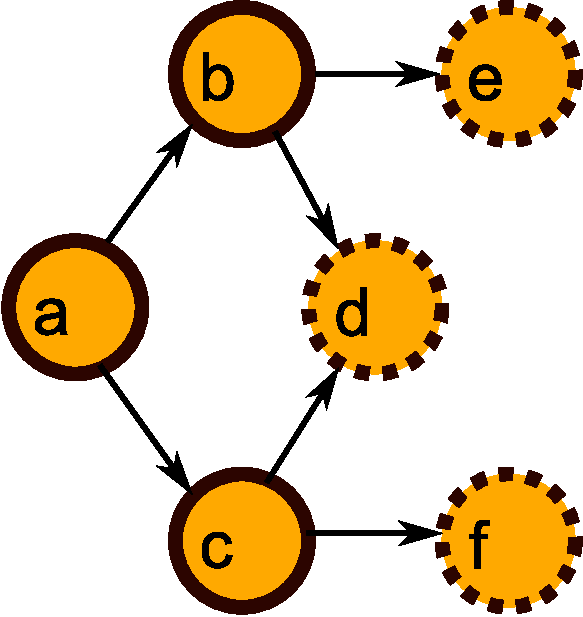
\includegraphics[width=4cm]{dependencies-one}
    \end{center}
    \caption{\small Dependency diagram for a single forecast cycle
    in a simple example system. Tasks $a$, $b$, and $c$ represent
    different forecast models, and $d$, $e$ and $f$ post processing or
    product generation tasks.}
    \label{fig-dep-one}
\end{figure}

Figure \ref{fig-dep-one} shows the task dependency diagram for a single
forecast cycle in a simple example system, which forms a {\em Directed
Acyclic Graph}. The graph is actually incomplete because it does not
show the intercycle dependencies that exist, at the least, between
consecutive runs of each forecast model (each new forecast starts from a
{\em background model state} generated by the previous forecast). But
if one cycle always completes before the next starts then any intercycle
dependencies are implicitly satisfied and can be ignored. In any
case, according to the diagram, each task may depend upon one or more
other upstream tasks, and one or more other downstream tasks may in turn
depend on it. A control system could therefore allow multiple parallel
streams of execution that branch when one task generates output for
several downstream tasks, and merge when one task takes input from
several upstream tasks. 
\begin{figure}
    \begin{center}
        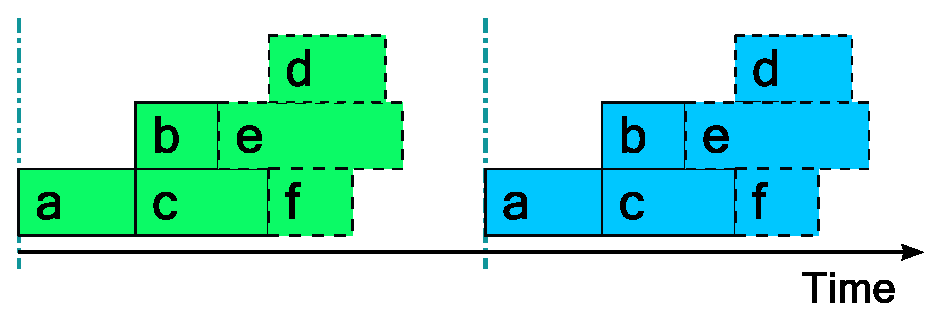
\includegraphics[width=8cm]{timeline-one}
    \end{center}
    \caption{\small Optimal job schedule for two consecutive cycles of
    the example system of Figure \ref{fig-dep-one}. Task execution
    times are represented by the horizontal extent of the task bars.}
    \label{fig-time-one}
\end{figure}
Figure \ref{fig-time-one} shows the optimal job schedule for two
consecutive cycles of the example system, given the execution times
represented by the horizontal extent of the task bars.  It is optimal in
the sense that each task is executed as soon as its dependencies are
satisfied. In reality, this means tasks will be queued for execution at
the earliest possible time; whether they actually run immediately is up
to the batch queue scheduler(s), but for the purposes of this paper we
can assume they will run immediately.  The vertical ordering of the task
bars is not meaningful, but a vertical section will cut through the
tasks executing in parallel at the time.

Perhaps the obvious design for a control system to manage this is a
Finite State Machine that enforces a predetermined but non-linear order
of task execution within each forecast cycle using hard coded sequencing
logic: {\em if task A has generated file X, and task B has finished,
then begin executing task C}, etc. This is easily understood and
straightforward to implement if the sequencing logic is not too
convoluted. In fact, as far as the author is aware all existing forecast
control systems are variations on this design, although it is difficult
to be sure because they are invariably system-specific in-house projects
that are not documented in the literature.\footnote{DAGMan, which is
part of the Condor distributed workload management system [REF:...] is a
generic metascheduler for job sets with dependencies, but it does not
appear to be suited to the type of continuously cycling system that will
be described below.}

\subsubsection{Design Deficiencies}

Finite State Machine controllers, as described above, have some serious
deficiencies. In addition to being highly system-specific, the hard
coded sequencing logic inevitably becomes convoluted with increasing
system complexity, which leads to inflexibility and fragility (consider
adding a new task with dependencies into an existing system). It is
possible to mitigate this somewhat by having the controller work at a
slightly higher level of abstraction on an external list of tasks rather
than using direct hard coding, but this makes it more difficult to fully
exploit the potential for parallism within the forecast cycle. Also,
such control systems cannot allow consecutive cycles to interleave when
the external driving data is available in advance, due to the assumption
that allows intercycle dependencies to be ignored: complete forecast
cycles must run strictly in sequence. This is a serious problem for
operational systems that, because of hardware limitations, have little
down time between cycles: catching up to real time operation after a
delay will take dramatically longer than necessary if complete cycles
have to run in sequence. The ability to run tasks from many cycles at
once, where dependencies allow, would also be extremely valuable for
parallel test systems catching up to the main operation, and to a lesser
extent during real time operation for certain kinds of complex
dependency (c.f.  EcoConnect's catchment model \dots), and when running
the entire system, or part thereof, over historical case study periods.  


\subsection{A New Approach} 

NIWA's EcoConnect operation, which motivated this work, is sufficiently
complex and computationally intensive, on current hardware, to warrant a
more flexible control system that is also able to interleave different
cycles for efficient catchup operation.  The only way to do this,
however, is to abandon, for task scheduling purposes, the concept of a
global ``forecast cycle'' and instead take proper account of {\em all}
dependencies regardless of forecast cycle.  While it may be possible in
principle to do this within a Finite State Machine, in practice the
additional sequencing logic would be prohibitively complex and convoluted. 

\begin{figure} \begin{center}
    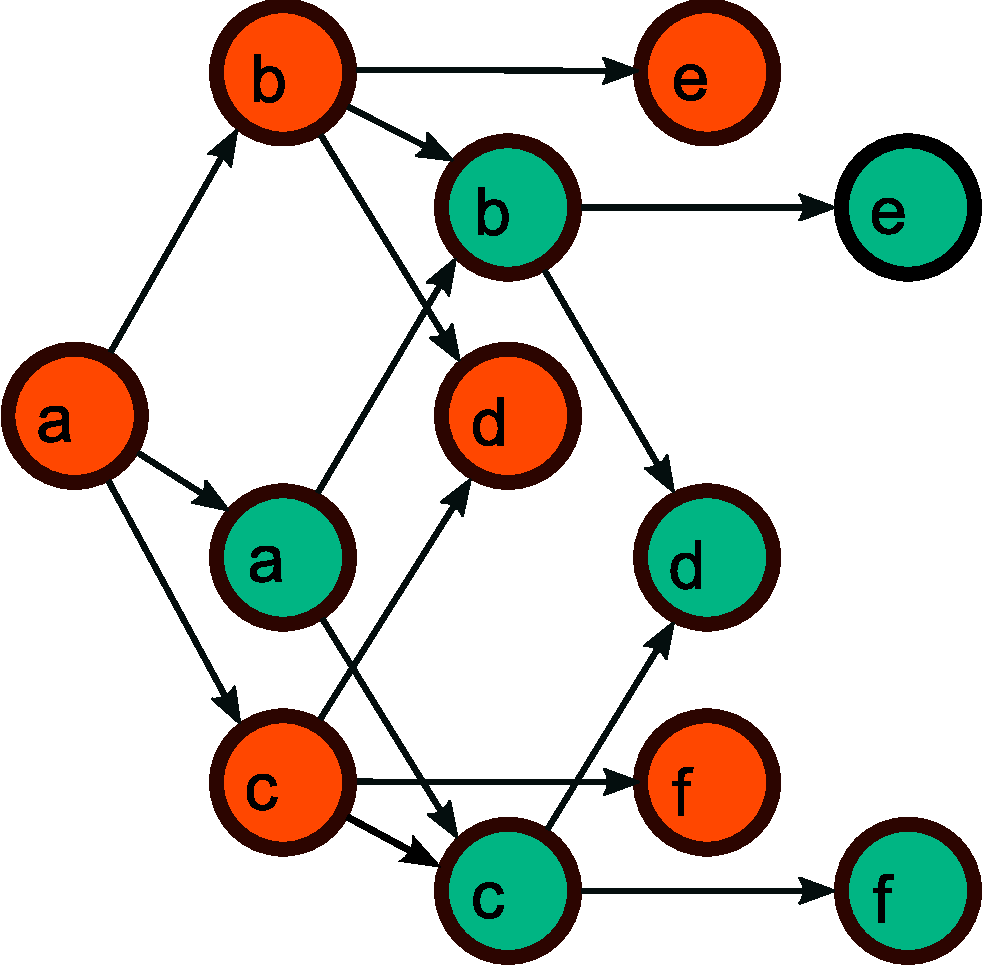
\includegraphics[width=6cm]{dependencies-two} \end{center}
    \caption{\small Diagram showing the dependencies for two consecutive
    cycles of our simple example system, with intercycle dependencies
    shown for the tasks that represent forecast models ($a$, $b$, and
    $c$).  Note that this is just a short section of a continuous
    system, and that more realistic systems can also include dependencies
    that span more than one forecast cycle.} 
    \label{fig-dep-two}
\end{figure}
Figure \ref{fig-dep-two} shows two cycles of the dependency
diagram for our example system, with intercycle dependencies included
(recall that tasks $a$, $b$, and $c$ represent forecast models, for
which each new forecast depends on a background state generated by the
previous forecast). While this example is sufficient to demonstrate
optimal metascheduling without a global forecast cycle, note that
the dependency diagram is really part of a continuous system (connected
to previous and subsequent cycles) and that real systems can be
considerably more complicated than this. For instance, the
intercycle dependence of forecast models that don't run in every
cycle would clearly span several cycles, and there may also be
intercycle dependencies between tasks of different kinds (c.f.\ the
EcoConnect catchment model's dependence on the regional weather model,
as described above). 

Figure \ref{fig-time-two} shows the optimal task schedule for the
example system, updated for the dependencies of Figure
\ref{fig-dep-two}, when the external driving data is available in
advance (for catchup operation, etc., as explained above).
\begin{figure} \begin{center} 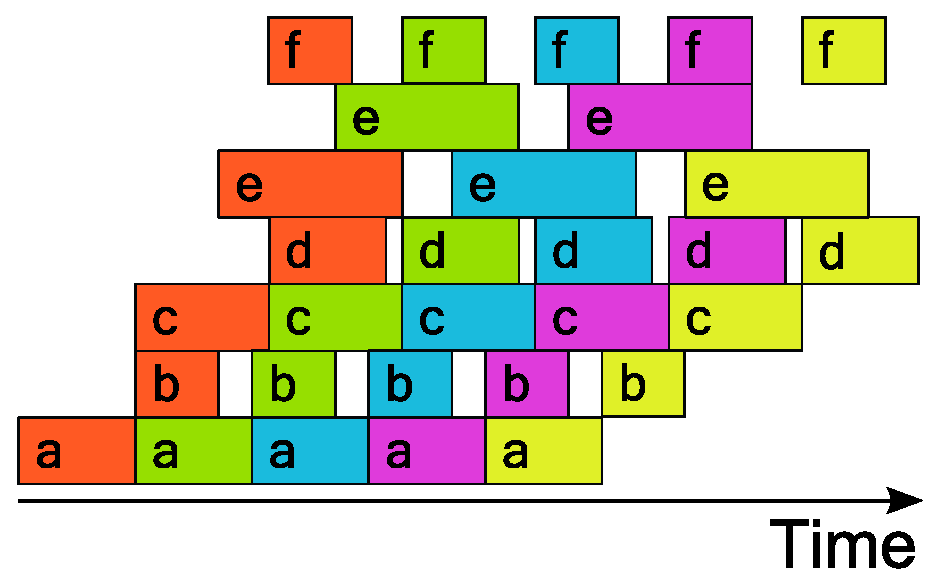
\includegraphics[width=8cm]{timeline-two}
\end{center} \caption{\small Optimal job schedule for tasks spanning
several consecutive cycles of our example system, with dependencies as
shown in Figure \ref{fig-dep-one}. Task execution times are represented
by the horizontal extent of the task bars.} \label{fig-time-two}
\end{figure} The initial task $a$, which has no upstream dependencies in
the same forecast cycle, can run continuously regardless of how much
downstream processing is yet to be completed in any previous cycle.
This is a big gain in itself as the initial forecast task(s) are
normally resource intensive atmosphere or ocean models. In reality these
tasks would actually depend on cotemporal (same reference time) upstream
tasks that wait on external input data, but these return immediately
when the external data is available in advance, so the argument still
holds. The other tasks can repeat at regular short intervals, for which
the interval gap is the difference between their own run length and the
maximum combined upstream run length of their upstream dependencies.
Task $c$ runs continuously, and consecutive instances of task $e$ can
actually overlap significantly. At any given time tasks from three
different cycles can run simultaneously, even for this very simple
system, and efficiency is clearly far in advance of the sequential
cycling schedule of Figure \ref{fig-time-one} (for which the time gap
between the two cycles should be shrunk to zero, for comparison). 

In the following sections we describe the implementation of a new
algorithm, based on task proxy objects that interact to negotiate
dependencies in real time, that can do optimal metascheduling for
continuously cycling forecasting systems, as represented in Figure
\ref{fig-time-two}. As the system catches up to real time and is again
constrained by availability of the external driving data it smoothly
transitions to a linear sequence of complete cycles as in Figure
\ref{fig-time-one}.  In addition, in contrast to the aforementioned
existing Finite State Machine controllers, the new method is completely
generic (i.e.\ not system-specific), extremely flexible, and widely
applicable.  


\section{Object Oriented Dynamic Metascheduling}

As explained in the introduction, in order to achieve optimal
metascheduling efficiency the concept of ``forecast cycle'' has to be
demoted, at least for scheduling purposes, from a globally incremented
system parameter to an independently incremented parameter of each
individual task. This prompted an Object Oriented control system design
in which proxy objects that represent the tasks, each with their own
``forecast reference time'', all interact regardless of reference time,
to negotiate dependencies at run time. The flexibility of this approach
is self-evident. Dynamic negotiation of dependencies means there is
absolutely no need for hardwired system-specific task sequencing logic,
and by means of object polymorphism\footnote{Polymorphism is the ability
of one type to appear as and be used like another type. In OOP languages
with inheritance, this usually refers to the ability to treat derived
class objects as if they were members of a base class so that, for
instance, a group of mixed-type objects can all be treated as members of
a common base class while retaining their specialized derived class
behaviour.} a control system can be designed that will, without
modification, automatically handle any conceivable new task so long as
it is derived from (inherits the properties of) the original task base
class. 

\subsection{Task Dependencies}

\subsection{Task Proxy Interaction}


\begin{comment}

Each task in a forecasting system has an associated {\em forecast
reference time}; for a forecast model this is the nominal forecast start
time, and for other tasks it is the reference time of the associated
forecast model.  And, in addition, each task type repeats on some
task-dependent interval. 

A task is ready to run when its upstream dependencies are satisfied,
usually by way other tasks generating its input files, so it is
important to consider what kinds of dependencies occur in the system.

However, there are also several kinds of non-cotemporal (different
reference time) dependence.  Forecast models generally depend on their
own previous instance, because one forecast generates the {\em
background model state} for the next.  In addition, some forecast models
may depend explicitly on earlier tasks of a different type, as well as
on their own previous instance.  Post processing tasks, on the other
hand, do not depend on their own previous instance, strictly speaking,
but they depend on cotemporal forecast models that do. EcoConnect's
hourly river flow forecasts, for example, take input from the most
recent previous regional weather forecast.  Finally, some tasks, such as
those that wait on external input data, and tide models, may have no
upstream dependencies at all.

 Non-forecast
model tasks can even overlap with their own previous instances, if the
opportunity arises (this occurs when a post processing task takes longer
to run than the delay between its upstream model starting and it
starting).  System throughput can be greatly increased by allowing tasks
from many different forecast cycles to run simultaneously where
dependencies allow.

This could be done by checking for the existence of required inputs
directly, or by monitoring the state of the other tasks that are known
to provide the inputs in each case (are they finished yet?).  

\subsection{Dynamic Metascheduling}

Dynamic Metascheduling is an object oriented approach to the problem.
Within the control program each task is represented by a self-contained
{\em task object} that knows nothing about other tasks in the system but
does know its own prerequisites (inputs) and outputs, and can interact
with other tasks to negotiate dependencies so that correct sequencing
emerges naturally at run time.  The entire sequencing problem is now
contained within the task interaction step, which is almost trivial
because it is completely indiscriminate: whenever any task changes
state, {\em each task} asks {\em all the others} if they can satisfy its
prerequisites with their completed outputs (it does not matter that most
of these interactions are destined to be fruitless). The control program
thus remains simple and generic, regardless of the number of tasks or
the complexity of their interdependencies; it simply manages a set of
tasks that are all individually configured as if they were to run in
isolation.\footnote{The system manager does of course have to ensure
that the configured task pool is self consistent, i.e.\ that each task's
prerequisites will be satisfied by some other task(s) in the system.}
The total absence of explicit sequencing logic makes this method
extremely flexible and extensible.\footnote{To extend the system, one
simply derives a new class definition that lists the new task's
prerequisites and outputs. The new task will automatically run at the
right time, i.e.\ when its prerequisites have been satisfied by some
other task(s) in the system.}

Dynamic sequencing can be viewed as a simulation of an interacting task
set in which the state of each {\em simulee} is tied to, and can
influence, that of the real task it represents.  This suggests a
powerful dummy mode of operation in which the simulation is divorced
from reality by replacing external tasks with an external dummy program
that masquerades as a real task by ``completing'' each of its outputs in
turn (i.e.\ it reports they are complete because, as far as the
controller is concerned, task outputs are just {\em messages}; more on
this below).  The control program cannot distinguish this from real
operations, so the dummy mode allows complete testing of the control
system for a given configured task set, without running any real tasks.


\subsection{{\em Sequenz}}

A dynamic sequencing controller would clearly be most naturally
implemented in an object oriented programming language, which provides
the tools for object construction and interaction.  We must also provide
the means for task objects to launch their external tasks when their
prerequisites are satisfied (e.g.\  by submission to a batch queue
scheduler on a task-dependent target machine), and for synchronization
of the internal states of task objects and the external tasks they
represent, via remote method calls or something similar.  Finally, the
generic description above assumes that task objects exist whenever they
are needed (for external task control and for interacting with other
dependent tasks), so we must devise a task management scheme governing
the creation and destruction of task objects, to ensure that this is the
case.

NIWA's EcoConnect Forecasting System, described above, is controlled by
an asynchronous dynamic sequencing implementation called {\em Sequenz},
implemented in object oriented Python and using the Python Remote Object
protocol ({\em Pyro}) for direct network communication between task
objects and the tasks they represent. It allows tasks from many
different forecast cycles to run at once, where dependencies allow,
transitions seamlessly from ``catchup'' or case study mode (where all
external input is available from the outset and much asynchronous
activity is therefore possible, e.g.\ after system downtime; in this
case) to normal real time operation, tasks can be switched on and off
while the controller is running, new tasks added without any change to
the main program, and the system can be restarted in arbitrarily complex
states after downtime.  It also features the powerful dummy mode
described above, for testing, and allows easy construction of ad hoc
parallel test systems feeding off the main operational system. Pyro also
enables efficient RPC-based remote control and system monitoring by
external programs.  Sequenz can be interfaced to existing models and
tasks with minimal overhead. 

The operation runs on heterogenous distributed
hardware, which includes a massively parallel supercomputer and several
Linux servers. 

\subsubsection{Applicability}

The dynamic sequencing concept is very general and could in principle be
implemented for any set of interdependent tasks. Sequenz, however, is
somewhat specialized toward cycling forecast systems, such as
EcoConnect, in which each task has an associated {\em reference time}
(generally the nominal forecast start time, or {\em analysis} time, of
the associated forecast model) that all task prerequisites and outputs
depend on in some way. and a set of valid times for each task type (e.g.\
the atmospheric model might run at 00, 06, 12, and 18 UTC each day,
while the river model runs hourly).  One-off task pools with no
particular time dependence, however, are much simpler than this, and it
would not be difficult to strip all reference time handling from the
program.

In addition, EcoConnect operates in a well defined environment so that,
for example, each task knows exactly what its input files look like
(filenaming conventions) and where to get them from (e.g.\ {\em task X}'s
output directory). Consequently, for file-based prerequisites, the
controller does not need to know the file's actual location or check for
its existence, because the external tasks already do that. It could,
however, easily be made to pass file locations between tasks so that all
input/output filenames and paths could be defined centrally in the
control program itself.  


\subsection{Alternatives}

As far as the author is aware, there are currently no other systems
available that can do general {\em asynchronous} sequencing, as
described in this paper.

In the planning stage, in addition to considering a Finite State Machine
design, as discussed above, we also considered new generation batch
queue schedulers (which now allow simple job dependencies), and use of
some kind of generic control framework.  Schedulers are still too
rudimentary for our purposes, however, and no generic control framework
that was obviously well suited came to light. In any case, the dynamic
sequencing design described in this paper simplifies the problem to such
an extent that it is unlikely any generic framework could compete.  


\section{Implementation}

To implement dynamic sequencing we need a specific {\em task management}
scheme that controls when tasks will be created and destroyed, and so
on. There are many options here; for instance: should tasks be created
all at once, in cotemporal batches, or one at a time as their
predecessors finish? The consequences of these choices must be evaluated
carefully, which isn't easy in light of the inherent complexity of
asynchronous operation. At the simpler end of the task management
spectrum we could, for example, create a whole month's worth of tasks at
once and let them interact until everything runs to completion.  Nothing
would run out of sequence, {\em but} system monitoring would be
difficult because of the sheer number of tasks involved, the end of the
month would present an artificial barrier to operations, tasks that lack
prerequisites would all want to run at once, and system restarts would
be overly complicated. 

\subsection{Main Algorithm}

The algorithm below operates on a single pool of interacting task
objects, has simple start up and continuous operation, and is relatively
easy to monitor (task objects exist by the time they are needed but not
for too long before that, and not for too long after they are finished). 

The simplicity of the dynamic sequencing algorithm is clear from the
following code listing, taken directly from the main program:

{\small
\noindent
\rule{5cm}{.2mm}
\begin{lstlisting}
# (startup initialization code omitted)

while True: # MAIN LOOP

   if task_base.state_changed:
       # PROCESS ALL TASKS whenever one has changed state
       # as a result of a remote task message coming in: 
       # interact, run, create new, and kill spent tasks
       #---
       task_pool.process_tasks()
       task_pool.dump_state()
       if task_pool.all_finished():
           clean_shutdown( "ALL TASKS FINISHED" )

    # REMOTE METHOD HANDLING; handleRequests() returns 
    # after one or more remote method invocations are 
    # processed (these are not just task messages, hence 
    # the use of task_base.state_changed above).
    #---
    task_base.state_changed = False
    pyro_daemon.handleRequests( timeout = None )

# END MAIN LOOP
\end{lstlisting}
}

\subsection{Details}

\subsubsection{Startup and Initialization}

An initial reference time and list of task object names are read in from
the config file, then each task object is created at the initial
reference time {\em or} at the first subsequent reference time that is
valid for the task type. Optionally, we can tell the controller to
reload the current state dump file (which may have been edited); this
will override the configured start time and task list. After startup,
new tasks are created only by {\em abdication} (below).

An initial run through the {\em task processing} code, by virtue of the
fact that the main loop starts with task processing, causes tasks with
no prerequisites (e.g.\ {\em downloader}) to enter the {\em running}
state and launch their external tasks immediately. Otherwise ({\em or}
if there are no tasks that lack prerequisites) nothing will happen.



\subsubsection{Creation of New Tasks}

New tasks are created by abdication, i.e.\ create $foo(T\negmedspace
+\negmedspace 1)$ if $foo(T)$ is {\em finished}.  Task abdication
ensures that $foo(T\negmedspace +\negmedspace 1)$ won't run before
$foo(T)$ finishes, without imposing explicit intercycle prerequisites
that would require special treatment at startup (when there is no
previous cycle).  It also ensures that tasks with no prerequisites, e.g.\
{\em downloader} and {\em nztide}, won't all try to run at once.
Tasks are not deleted immediately on abdication (see below).


\subsubsection{Task Interaction} 

Each task keeps track of which of its postrequisites are completed, and
asks the other tasks if they can satisfy any of its prerequisites.  The
fact that task objects do not need to know who is supposed to satisfy
their prerequisites (because they can ask, indiscriminately, every other
task in the system) makes the task interaction (sequencing!) algorithm
almost trivial. The fact that most of these interactions are fruitless
is of no consequence. 

{\small
\noindent
\rule{5cm}{.2mm}
\begin{lstlisting}
class task_pool( Pyro.core.ObjBase ):
    # ...
    def interact( self ):
        # get each task to ask all the others if 
        # they can satisfy its prerequisites
        #--
        for task in self.tasks:
            task.get_satisfaction( self.tasks )
    # ...
\end{lstlisting}
}

\subsubsection{Running Tasks}

Each task object can launch its associated external task, and enter the
{\em running} state if its prerequisites are all satisfied, any existing
older tasks of the same type are already {\em finished}, and fewer than
{\em MAX\_ RUNAHEAD} finished tasks of the same type still exist (this
stops tasks with no prerequisites from running ahead indefinitely).

\subsubsection{Pyro Remote Method Calls}

The Pyro request handling loop executes remote method calls coming in
from external tasks, and returns after at least one call was handled.
Pyro must be run in non-default single-threaded mode (see Appendix
\ref{pyro-appendix}).

\subsubsection{Dumping State} 

The current state (waiting, running, or finished) of each task is
written out to the {\em state dump file}.  This provides a running
snapshot of the system as it runs, and just prior to shutdown or
failure. The controller can optionally start up by loading the state
dump (which can be edited first). Any 'running' tasks are reloaded in
the 'waiting' state.

\subsubsection{Removing Spent Tasks} 

A task is spent if it finished {\em and} no longer needed to satisfy the
prequisites of any other task. Most tasks are only needed by other
cotemporal downstream tasks; these can be removed when they are finished
{\em and} older than the oldest non-finished task. For rare cases that
are needed by tasks in later reference times (e.g.\ nzlam post
processing: multiple hourly topnet tasks need the same most recent
previously finished 06 or 18Z nzlam post processing task), each
non-finished task reports its {\em cutoff reference time} which is the
oldest reference time that may contain tasks still needed to satisfy its
own prerequisites (if it is waiting) or those of its immediate
post-abdication successor (if it is running already), then the task
manager can then kill any finished tasks that are also older than the
oldest task cutoff time.

\subsubsection{Removing Lame Tasks} 

Tasks that will never run (because their prerequisites cannot be
satisfied by any other task in the system) are removed from the {\em
oldest batch} of tasks.  If not removed they would prevent the spent
task deletion algorithm from working properly. Lame tasks can only be
detected in the oldest task batch; in younger batches some tasks may yet
appear as their predecessors abdicate.

Lame tasks are abdicated rather than just deleted, because their
descendents will not necessarily be lame: e.g.\ if the system is started
at 12Z with topnet turned on, all topnet tasks from 12Z through 17Z will
be valid but lame, because they will want to take input from a
non-existent nzlam\_post from 06Z prior to startup. However, the
presence of lame tasks may indicate user error: e.g.\ if you forget
to turn on task type $foo$ that supplies input to task type $bar$,
any instance of $bar$ will be lame.


\subsection{Dummy Mode}

Dummy mode allows complete testing of the control system without running
any real external tasks\footnote{The only difference between dummy mode
and real operation, as far as the controller is concerned, is that
external dummy tasks are not delayed by resource contention.}. When it
is ready to run, a task object will launch an external dummy program
that (i) gets a list of postrequisites from the parent task object and
then (ii) reports back that each one is satisfied at the (estimated)
right time relative to an accelerated dummy clock. Dummy tasks therefore
complete in approximately the same dummy clock time as the real tasks do
in real time. An initial dummy clock offset relative to the initial
reference time can also be specified, which allows simulation of the
transition between catchup and real time operation. Log messages are
stamped with dummy clock time instead of real time.

The same script is used for all external dummy tasks but it has special
behaviour in certain cases: the dummy downloader ``waits for incoming
files'' until 3:15 past its reference time, and the dummy topnet ``waits
for stream flow data'' until 0:15 past its reference time.

The dummy clock can be bumped forward a number of hours by remote
control, while the system is running. This affects the postrequisite
timing of running tasks correctly, but if it causes a running task to
finish immediately the next task in line will still start from the
beginning no matter how big the bump.


\appendix

\section{Essential OOP Concepts}

The simplicity of the dynamic sequencing implementation in {\em sequenz}
is critically dependent on the {\em polymorphic} nature of the {\em task
objects} in the program.  This section contains a minimal introduction
to these Object Oriented Programming concepts.  Refer to any OOP
reference for more detail.

\subsection{Classes and Objects}

A {\em class} is essentially a generalisation of {\em data type} to
include {\em behaviour} (i.e.\ functions or {\em methods}) as well as
state.  {\em Objects} are more or less self contained {\em instances} of
a class. For example, a $shape$ class could define a $position$ data
member that describes the location of each shape object, a $move()$
method that causes a shape object to alter its position, and a $draw()$
method that causes it to display itself in the right place on screen.

\subsection{Inheritance}

A {\em derived class} or {\em subclass} inherits the properties (methods
and data members) of a {\em base class}. It can also {\em override}
specific base class properties, or add new properties that aren't
present in the base class. Calling a particular method on an object
invokes the object's own class method if one is defined, otherwise the
immediate base class is searched, and so on down to the root of the
inheritance graph. 

For example, we could derive a $circle$ class from $shape$, adding a
`radius' data member and overriding the $draw()$ to get circle objects
to display themselves as actual circles.  Because we didn't override the
$move()$ method, calling $circle.move()$ would invoke the base class
method, $shape.move()$. 


\subsection{Polymorphism}

Polymorphism is the ability of one type to appear as and be used like
another type.  In OOP languages with inheritance, this usually refers to
the ability to treat derived/sub-class objects as if they were members
of a base class.  In particular, a group of mixed-type objects can all
be treated as members of a common base class. For example, we could
construct a list of $shape$ objects from $circles$, $triangles$, and
$squares$; calling $[list member].draw()$ will invoke the right derived
class $draw()$. This is a very powerful mechanism because {\em it allows
unmodified old code to call new code}: if we later derive an entirely
new kind of shape ($hexagon$, say) with it's own unique behaviour, the
existing program, without modification, will process the new objects in
the proper hexagon-specific way.


\section{Threading in Pyro} \label{pyro-appendix}

With Pyro in {\em single threaded mode}, \verb#handleRequests()# returns
after {\em either} a timeout has occurred {\em or} at least one request
(i.e.\ remote method call) was handled. With \verb#timeout = None# this
allows us to process tasks {\em only} after remote method invocations
come in.  Further, we can detect the remote calls that actually change
task states, and thereby drop into the task processing code only when
necessary, which minimizes non-useful output from the task processing
loop (e.g.\ in dummy mode there are a lot of remote calls on the dummy
clock object, which does not alter tasks at all). 

In {\em multithreaded mode}, \verb#handleRequests()# returns immediately
after creating a new request handling thread for a single remote object
and thereafter remote method calls on that object come in asynchronously
in the dedicated thread. This is not good for the dynamic sequencing
algorithm because tasks are only set running in the task processing
block which can be delayed while \verb#handleRequests()# blocks waiting
for a new connection to be established even as messages that warrent
task processing are coming in on existing connections. The only way
around this is to do task processing on \verb#handleRequests()# timeouts
which results in a lot of unnecessary task processing when nothing
important is happening.


\section{YET TO BE DOCUMENTED}

\begin{itemize}
 \item usage
 \item logging
 \item debugging
 \item adding new task definitions
 \item system monitors
 \item remote control: 
    \begin{itemize}
    \item clean shutdown of pyro
    \item bumping the dummy clock forward
    \end{itemize}
 \item external task messaging interface script
 \item dummying out tasks in real mode
 \item how to set up partial parallel test systems
\end{itemize}

\section{Miscellaneous Notes}

(To be incorporated into the main documentation, or deleted).

\subsection{catchup mode}

Note that ``correct model sequencing'' is not equivalent to ``orderly
generation of products by reference time''.  Nzlam can run continuously,
regardless of the downstream processing that depends on it.

Catchup mode is now task-dependent, rather than a property of the whole
system (as it is if only tasks from the same reference time can run at
once).  Where this matters, it can be detected by the relevant external
task. E.g.\ if the external topnet(T) task starts up at real time t
greater than the stream flow data time for T (i.e.\ $T+15$ min), i.e.\ the
required stream flow data is already available, then we're still in
catchup. If, on the other hand, the topnet task finds that it has to
wait for its stream flow data time to arrive, then we're caught up to
real time.  This matters because topnet is allowed to run ahead by a
different amount of time depending on whether we're in catchup mode or
not.


\subsection{controlling when a task executes}

\begin{itemize}
 \item  prerequisites
 \item artificial prerequisites (e.g.\ make nztide depend on nzlam)
 \item delayed instantiation (a task can't run if it doesn't exist yet).
 \item other contraints based on, for example, the number of previous
 instances that still exist in the system.
\end{itemize}


\subsection{fuzzy prequisites}

{\em Exact prerequisites} (most tasks): times are specified exactly,
relative to the task's own reference time.  E.g.\ {\em file foo\_{T}.nc
ready} where T is the task's reference time.

{\em Fuzzy prerequisites} (topnet): a time boundary is specified
relative to the task's own reference time; any task with a reference
time greater than or equal to the boundary time can satisify the
prerequisite.

\subsection{Task Messaging}

To the task objects, outputs are just {\em messages} indicating that the
external task has reached a significant waypoint, such as generation of
a particular output file.

\section{To Do}

\begin{itemize}

\item
 retrofit proper exception handling throughout (currently used sparsely and 
  inconsistently)

\item
 potential bug in the free task class: will never run if too many
 previous instances exist that are newer than the task deletion cutoff

\item
 remote logging from messaging and dummy task scripts, in case the
 controller itself is dead.

\end{itemize}


\end{comment}

\end{document}

